\section{Character-based convolutional encoder for NMT}
\label{sec:char_enc}
In Assignment 4, we used a simple lookup method to get the representation of a word.
If a word is not in our pre-defined vocabulary, then it is represented as the \texttt{<UNK>} token (which has its own embedding).

\begin{figure}[h]
    \captionsetup{width=0.8\textwidth}
    \begin{center}
        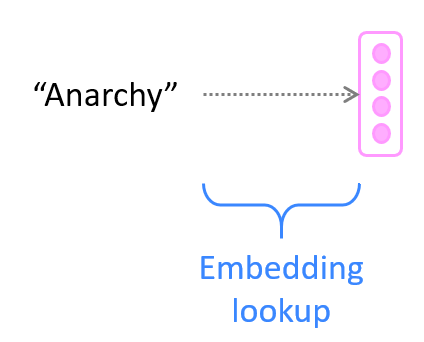
\includegraphics[width=0.25\textwidth]{images/word-embedding.PNG}
        \caption{Lookup-based word embedding model from Assignment 4, which produces a word embedding of length $e_\text{word}$.}
        \label{fig:word-emb}
    \end{center}
\end{figure}

In this section, we will first describe a method based on Kim et al.'s work in \textit{Character-Aware Neural Language Models},\footnote{Character-Aware Neural Language Models, Kim et al., 2016. \url{https://arxiv.org/abs/1508.06615}} then we'll implement it. Specifically, we'll replace the `Embedding lookup' stage in Figure \ref{fig:word-emb} with a sequence of more involved stages, depicted in Figure \ref{fig:char-emb}.

\begin{figure}[h!]
    \captionsetup{width=0.8\textwidth}
    \begin{center}
        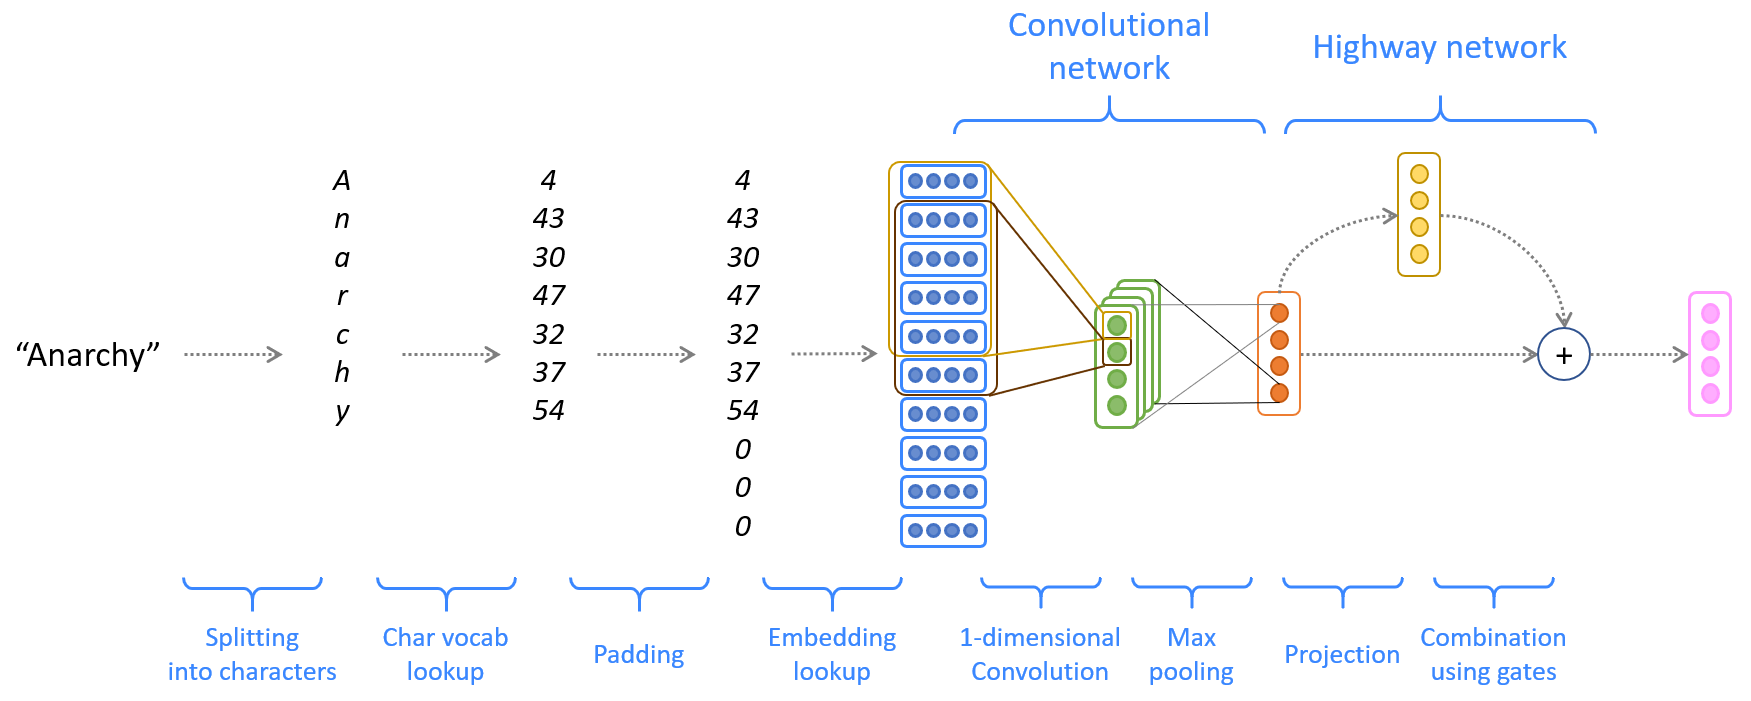
\includegraphics[width=0.9\textwidth]{images/embedding.PNG}
        \caption{Character-based convolutional encoder, which ultimately produces a word embedding of length $e_\text{word}$.}
        \label{fig:char-emb}
    \end{center}
\end{figure}
\newpage
\subsection*{Model description}
The model in Figure \ref{fig:char-emb} has four main stages, which we'll describe for a \textit{single example} (not a batch):
\begin{enumerate}[(a)]
    \item \textbf{Convert word to character indices}.
    We have a word $x$ (e.g. \texttt{Anarchy} in Figure \ref{fig:char-emb}) that we wish to represent. 
    Assume we have a predefined `vocabulary' of characters (for example, all lowercase letters, uppercase letters, numbers, and some punctuation).
    By looking up the index of each character, we can thus represent the length-$l$ word $x$ as a vector of integers:
    \begin{equation}
        \bx = [c_1, c_2, \cdots, c_{l}] \in \Int^l
    \end{equation}
    where each $c_i$ is an integer index into the character vocabulary. 

    \item \textbf{Padding and embedding lookup}.
    Using a special \texttt{<PAD>} `character', 
    we pad (or truncate) every word so that it has length $m_\text{word}$ (this is some predefined hyperparameter representing maximum word length):
    \begin{equation}
        \bx_{\text{padded}} = [c_1, c_2, \cdots, c_{m_{\text{word}}}] \in \Int^{m_\text{word}}
    \end{equation}
    For each of these characters $c_i$, we lookup a dense character embedding (which has shape $e_\text{char}$). This yields a tensor $\bx_\text{emb}$:
    \begin{equation}
        \bx_\text{emb} = \text{CharEmbedding}(\bx_{\text{padded}}) \in \Real^{m_{\text{word}}\times e_\text{char}}    
    \end{equation}
    We'll reshape $\bx_\text{emb}$ to obtain $\bx_{\text{reshaped}} \in \Real^{e_\text{char} \times m_\text{word}}$ before feeding into the convolutional network.\footnote{Necessary because the PyTorch Conv1D function performs the convolution only on the \textit{last} dimension of the input.}
    \item \textbf{Convolutional network}.
        To combine these character embeddings, we'll use 1-dimensional convolutions (the pages from 16 to 25 of this slide\footnote{\url{https://nlp.seas.harvard.edu/slides/aaai16.pdf}} can be helpful to understand 1-d convolutions). The convolutional layer has two hyperparameters:\footnote{We assume no padding is applied and the stride is 1.} the kernel size $k$ (also called window size), which dictates the size of the window used to compute features, and the number of filters $f$ (also called number of output features or number of output channels). 
    The convolutional layer has a weight matrix $\bW \in \Real^{f \times e_\text{char} \times k}$ and a bias vector $\bb \in \Real^f$.
    \newline
    
    To compute the $i^\text{th}$ output feature (where $i \in \{1,\dots,f\}$) for the $t^\text{th}$ window of the input, the convolution operation is performed between the input window\footnote{In the notation $(\bx_\text{reshaped})_{[:, \> t:t+k-1]}$, the range $t:t+k-1$ is \textit{inclusive}, i.e. the width-$k$ window $\{t,t+1,\dots,t+k-1\}$.} $(\bx_\text{reshaped})_{[:, \> t:t+k-1]} \in \Real^{e_\text{char} \times k}$ and the weights $\bW_{[i, :, :]} \in \Real^{e_\text{char} \times k}$, and the bias term $\bb_i \in \Real$ is added:
    \begin{equation}
        (\bx_\text{conv})_{i, t} = \texttt{sum} \left( \bW_{[i, :, :]} \odot (\bx_\text{reshaped})_{[:, \> t:t+k-1]} \right) + \bb_i \quad \in \Real
    \end{equation}
    where $\odot$ is elementwise multiplication of two matrices with the same shape and \texttt{sum} is the sum of all the elements in the matrix.
    This operation is performed for every feature $i$ and every window $t$, where $t \in \{1,\dots,m_\text{word}-k+1\}$. Overall this produces output $\bx_\text{conv}$: 
    \begin{equation}
        \bx_{\text{conv}} = \text{Conv1D}(\bx_{\text{reshaped}})
        \in \Real^{f \times (m_\text{word}-k+1)}
    \end{equation}
    For our application, we'll set $f$ to be equal to $e_\text{word}$, the size of the final word embedding for word $x$ (the rightmost vector in Figure \ref{fig:char-emb}). Therefore, 
    \begin{equation}
        \bx_{\text{conv}} \in \Real^{e_\text{word} \times (m_\text{word}-k+1)}
    \end{equation}
    Finally, we apply the ReLU function to $\bx_{\text{conv}}$, then use max-pooling to reduce this to a single vector $\bx_{\text{conv\_out}} \in \Real^{e_\text{word}}$, which is the final output of the Convolutional Network:
    \begin{equation}
        \bx_\text{conv\_out} = \text{MaxPool}( \text{ReLU}(\bx_{\text{conv}}))  \in \Real^{e_\text{word}}
    \end{equation}
    Here, MaxPool simply takes the maximum across the second dimension. Given a matrix $M \in \Real^{a\times b}$, then $\text{MaxPool}(M)\in \Real^a$ with $\text{MaxPool}(M)_i = \max_{1\le j \le b} M_{ij}$ for $i \in \{1,\dots,a\}$.

    \item \textbf{Highway layer and dropout.}
    As mentioned in Lectures 7 and 11, Highway Networks\footnote{Highway Networks, Srivastava et al., 2015. \url{https://arxiv.org/abs/1505.00387}} have a skip-connection controlled by a dynamic gate. Given the input $\bx_\text{conv\_out} \in \Real^{e_\text{word}}$, we compute:
    \begin{align}
        \bx_{\text{proj}} &= \operatorname{ReLU}(\bW_{\text{proj}} \bx_\text{conv\_out} + \bb_{\text{proj}}) &\in \Real^{e_\text{word}} \\
        \bx_{\text{gate}} &= \sigma(\bW_\text{gate} \bx_\text{conv\_out} + \bb_\text{gate}) &\in \Real^{e_\text{word}}
    \end{align}
    where the weight matrices $\bW_\text{proj}, \bW_\text{gate} \in \mathbb{R}^{e_\text{word} \times e_{word}}$ and bias vectors $\bb_\text{proj}, \bb_\text{gate} \in \mathbb{R}^{e_\text{word}}$. 
    Next, we obtain the output $\bx_\text{highway}$ by using the gate to combine the projection with the skip-connection:
    \begin{equation}
    \bx_\text{highway} = \bx_\text{gate} \odot \bx_\text{proj} + (1-\bx_\text{gate}) \odot \bx_\text{conv\_out} \in \Real^{e_\text{word}}
    \end{equation}
    where $\odot$ denotes element-wise multiplication.
    Finally, we apply dropout to $\bx_\text{highway}$:
    \begin{equation}
        \bx_\text{word\_emb} = \text{Dropout}(\bx_\text{highway}) \in \Real^{e_\text{word}}
    \end{equation}
\end{enumerate}
We're done! $\bx_\text{word\_emb}$ is the embedding we will use to represent word $x$ -- this will replace the lookup-based word embedding we used in Assignment 4.
\newpage

\subsection*{{\color{red} Setting up your Virtual Machine}}
You can use the same VM and environment that you set up in A4.  Simply activate the environment like this:
\begin{lstlisting}
$ conda activate XCS224N
\end{lstlisting}
In case you need to reinstall your environment on a fresh VM, here are the instructions from A4:

Follow the instructions in the \href{https://docs.google.com/document/d/10J520Vnb1LnAMo0qgSYpG5cEEbomqQ371NIqg1IAv-4/edit?usp=sharing}{XCS224N Azure Guide} in order to create your VM instance. Though you will need the GPU to train your model, we strongly advise that you first develop the code locally and ensure that it runs, before attempting to train it on your VM. GPU time is expensive and limited. It takes approximately \textbf{8-12 hours} to train the system. We don't want you to accidentally use all your GPU time for the assignment, debugging your model rather than training and evaluating it. Finally, \textbf{make sure that your VM is turned off whenever you are not using it.}

In order to run the model code on your VM, please run the following command to create the proper virtual environment like this (You did this at the beginning of the course on your local computer):

\begin{lstlisting}
$ conda env create --file environment.yml
\end{lstlisting}

Next, you need to install GPU-specific dependencies on your VM.  First, activate the |XCS224N| environment you just created.  Then install the dependencies like this:

\begin{lstlisting}
$ conda activate XCS224N
(XCS224N)$ conda install --file gpu_requirements.txt
\end{lstlisting}

For local development and testing, you can feel free to continue to using the same |XCS224N| environment you've used for all the assignments so far.

\subsection*{Implementation}
In the remainder of Section \ref{sec:char_enc}, we will be implementing the character-based encoder in our NMT system.
Though you could implement this on top of your own Assignment 4 solution code, for simplicity and fairness we have supplied you\footnote{A4 implementation is included in the A5 starter code} with a full implementation of the Assignment 4 word-based NMT model (with some modifications); this is what you will use as a basis for your Assignment 5 code. 

You will not need to use your VM until Section 2 -- the rest of this section can be done on your local machine.

Let's implement the entire network specified in Figure \ref{fig:char-emb}, from left to right.

\begin{enumerate}[(a)]
    \item \points{1a} In \texttt{src/submission/vocab.py}, implement the method \texttt{words2charindices()} (hint: copy the structure of \texttt{words2indices()}) to convert each character to its corresponding index in the character-vocabulary. This corresponds to the first two steps of Figure \ref{fig:char-emb} (splitting and vocab lookup).

    \item \points{1b} Implement \texttt{pad\_sents\_char()} in \texttt{src/submission/utils.py}, similar to the version for words. This method should pad at the character and word level. 
    All words should be padded/truncated to max word length $m_\text{word}=21$, and all sentences should be padded to the length of the longest sentence in the batch.
    A padding word is represented by $m_\text{word}$ \texttt{<PAD>}-characters.

    \item \points{1c} Implement \texttt{to\_input\_tensor\_char()} in \texttt{src/submission/vocab.py} to connect the previous two parts: use both methods created in the previous steps and convert the resulting padded sentences to a torch tensor. \textbf{Ensure you reshape the dimensions} so that the output has shape: (\texttt{max\_sentence\_length}, \texttt{batch\_size}, \texttt{max\_word\_length}) so that we don't have any shape errors downstream! 

    \item \label{qn:highway} In the empty file \texttt{src/submission/highway.py}, implement the highway network as a \texttt{nn.Module} class called \texttt{Highway}.\footnote{If you're unsure how to structure a \texttt{nn.Module}, you can start here: \url{https://pytorch.org/tutorials/beginner/examples_nn/two_layer_net_module.html}. After that, you could look at the many examples of \texttt{nn.Modules} in Assignments 3 and 4.} 
    \begin{itemize}
        \item Your module will need a \texttt{\_init\_()} and a \texttt{forward()} function (whose inputs and outputs you decide for yourself).
        \item The \texttt{forward()} function will need to map from $\bx_\text{conv\_out}$ to $\bx_\text{highway}$.
        \item Note that although the model description above is not batched, your \texttt{forward()} function should operate on batches of words.
        \item Make sure that your module uses two \texttt{nn.Linear} layers.
    \end{itemize}
    There is no provided sanity check for your \texttt{Highway} implementation -- instead, you will now write your own code to thoroughly test your implementation. 
    You should do whatever you think is sufficient to convince yourself that your module computes what it's supposed to compute. 
    Possible ideas include (and you should do multiple):
    \begin{itemize}
        \item Write code to check that the input and output have the expected shapes and types. Before you do this, make sure you've written docstrings for \texttt{\_init\_()} and \texttt{forward()} -- you can't test the expected output if you haven't clearly laid out what you expect it to be!
        \item Print out the shape of every intermediate value; verify all the shapes are correct.
        \item Create a small instance of your highway network (with small, manageable dimensions), manually define some input, manually define the weights and biases, manually calculate what the output should be, and verify that your module does indeed return that value.
        \item Similar to previous, but you could instead print all intermediate values and check each is correct.
        \item If you can think of any `edge case' or `unusual' inputs, create test cases based on those.
    \end{itemize}
        
    \item \label{qn:cnn}
    In the empty file \texttt{src/submission/cnn.py}, implement the convolutional network as a \texttt{nn.Module} class called \texttt{CNN}.
    \begin{itemize}
        \item Your module will need a \texttt{\_init\_()} and a \texttt{forward()} function (whose inputs and outputs you decide for yourself).
        \item The \texttt{forward()} function will need to map from $\bx_\text{reshaped}$ to $\bx_\text{conv\_out}$.
        \item Note that although the model description above is not batched, your \texttt{forward()} function should operate on batches of words.
        \item Make sure that your module uses one \texttt{nn.Conv1d} layer (this is important for the autograder).
        \item Use a kernel size of $k=5$.
    \end{itemize}

Run the following to create the correct vocab files:
\begin{lstlisting}
(XCS224N)$ sh run.sh vocab
\end{lstlisting}

    \item \points{1f} Write the \texttt{\_\_init\_\_()} and \texttt{forward()} functions for the \texttt{ModelEmbeddings} class in \\
    \texttt{src/submission/model\_embeddings.py}.\footnote{Note that in this assignment, the full NMT model defines two \texttt{ModelEmbeddings} objects (one for source and one for target), whereas in Assignment 4, there was a single \texttt{ModelEmbeddings} object that contained two \texttt{nn.Embedding} objects (one for source and one for target).} 
    \begin{itemize}
        \item The \texttt{forward()} function must map from $\bx_\text{padded}$ to $\bx_\text{word\_emb}$ -- note this is for whole batches of sentences, rather than batches of words.
        \item You will need to use the \texttt{CNN} and \texttt{Highway} modules you created.
        \item Don't forget the dropout layer! Use 0.3 dropout probability.
        \item Your \texttt{ModelEmbeddings} class should contain one \texttt{nn.Embedding} object (this is important for the autograder).
        \item Remember that we are using $e_\text{char}=50$.
        \item Depending on your implementation of \texttt{CNN} and \texttt{Highway}, it's likely that you will need to reshape tensors to get them into the shape required by \texttt{CNN} and \texttt{Highway}, and then reshape again to get the final output of \texttt{ModelEmbeddings.forward()}.
    \end{itemize}
    
    The majority of the 12 points are awarded based on a hidden autograder. Though we don't require it, you should check your implementation using techniques similar to what you did in (\ref{qn:highway}) and (\ref{qn:cnn}), before you do the `small training run' check in (\ref{qn:run_tiny_enc}). 

    \item \points{1g}
    In \texttt{src/submission/nmt\_model.py}, complete the \texttt{forward()} method to use character-level padded encodings instead of word-level encodings.
    This ties together your \texttt{ModelEmbeddings} code with the preprocessing code you wrote. Check your code!
    
    \item \points{1h} \label{qn:run_tiny_enc} \textbf{On your local machine}, confirm that you're in the proper conda enironment then execute the following command. 
    This will train your model on a very small subset of the training data, then test it. Your model should overfit the training data.
\begin{lstlisting}
(XCS224N)$ sh run.sh train_local_q1
(XCS224N)$ sh run.sh test_local_q1
\end{lstlisting}

    Running these should take around 5 minutes (but this depends on your local machine). 
    You should observe the average loss go down to near 0 and average perplexity on train and dev set go to 1 during training. Once you run the test, you should observe BLEU score on the test set higher than 99.00. 
    If you don't observe these things, you probably need to go back to debug!

\end{enumerate}
